\documentclass[12pt,a4paper]{article}
\usepackage[utf8]{inputenc}
\usepackage[english]{babel}

\usepackage{amsmath}
\usepackage{amsfonts}
\usepackage{amssymb}

\usepackage{graphicx}
\usepackage{caption}
\usepackage{subcaption}
\usepackage{lmodern}
\usepackage{tikz}
\usepackage{titlesec}
\usepackage{environ}
\usepackage{xcolor}
\usepackage{fancyhdr}
\usepackage[colorlinks = true, linkcolor = black]{hyperref}
\usepackage{xparse}
\usepackage{enumitem}
\usepackage{comment}
\usepackage{wrapfig}
\usepackage[capitalise]{cleveref}

\usepackage[left=2cm,right=2cm,top=2cm,bottom=2cm]{geometry}
\usepackage{multicol}
\usepackage[indent=0pt]{parskip}

\newcommand{\spaceP}{\vspace*{0.5cm}}
\newcommand{\Span}{\mathrm{Span}\,}
\newcommand{\range}{\mathrm{range}\,}
\newcommand{\ra}{\rightarrow}

%% Redefining sections
\newcommand{\sectionformat}[1]{%
    \begin{tikzpicture}[baseline=(title.base)]
        \node[rectangle, draw] (title) {#1};
    \end{tikzpicture}
    
    \noindent\hrulefill
}

\newif\ifhNotes 

\hNotesfalse

\ifhNotes
	\newcommand{\hideNotes}[1]{%
	\phantom{#1}
	}
	\newcommand{\hideNotesU}[1]{%
	\underline{\hspace{1mm}\phantom{#1}\hspace{1mm}}
	}
\else
	\newcommand{\hideNotes}[1]{#1}
	\newcommand{\hideNotesU}[1]{\textcolor{blue}{#1}}
\fi

% default values copied from titlesec documentation page 23
% parameters of \titleformat command are explained on page 4
\titleformat%
    {\section}% <command> is the sectioning command to be redefined, i. e., \part, \chapter, \section, \subsection, \subsubsection, \paragraph or \subparagraph.
    {\normalfont\large\scshape}% <format>
    {}% <label> the number
    {0em}% <sep> length. horizontal separation between label and title body
    {\centering\sectionformat}% code preceding the title body  (title body is taken as argument)

%% Set counters for sections to none
\setcounter{secnumdepth}{0}

%% Set the footer/headers
\pagestyle{fancy}
\fancyhf{}
\renewcommand{\headrulewidth}{0pt}
\renewcommand{\footrulewidth}{2pt}
\lfoot{P.-O. Paris{\'e}}
\cfoot{MATH 241}
\rfoot{Page \thepage}

%% Defining example environment
\newcounter{example}[section]
\NewEnviron{example}%
	{%
	\noindent\refstepcounter{example}\fcolorbox{gray!40}{gray!40}{\textsc{\textcolor{red}{Example~\theexample.}}}%
	%\fcolorbox{black}{white}%
		{  %\parbox{0.95\textwidth}%
			{
			\BODY
			}%
		}%
	}

% Theorem environment
\NewEnviron{theorem}%
	{%
	\noindent\refstepcounter{example}\fcolorbox{gray!40}{gray!40}{\textsc{\textcolor{blue}{Theorem~\theexample.}}}%
	%\fcolorbox{black}{white}%
		{  %\parbox{0.95\textwidth}%
			{
			\BODY
			}%
		}%
	}

\NewEnviron{notes}%
	{%
	\noindent \fcolorbox{gray!40}{gray!40}{\textsc{\textcolor{blue}{Solution.}}}%
	%\fcolorbox{black}{white}%
		{  %\parbox{0.95\textwidth}%
			{
			\textcolor{blue}{%
			\BODY
			}
			}%
		}%
	}
%%% Ignorer les notes
\excludecomment{notes}

%%%%
\begin{document}
\thispagestyle{empty}

\begin{center}
\vspace*{2.5cm}

{\Huge \textsc{Math 241}}

\vspace*{2cm}

{\LARGE \textsc{Chapter 3}} 

\vspace*{0.75cm}

\noindent\textsc{Section 3.9: Antiderivatives}

\vspace*{0.75cm}

\tableofcontents

\vfill

\noindent \textsc{Created by: Pierre-Olivier Paris{\'e}} \\
\textsc{Spring 2023}
\end{center}

\newpage

\section{Definition}
A function $F$ is an \textbf{antiderivative} of a function $f$ if $F'(x) = f(x)$.

\vspace*{16pt}

\begin{example}
Find an antiderivative of the following functions.
\begin{multicols}{3}
	\begin{enumerate}[label=\textbf{(\alph*)}]
	\item $f(x) = x^2$.
	\item $g(x) = 3x^3 + \cos (x)$.
	\item $h(x) = x^{2/3} + 4 \sec^2 (x)$.
	\end{enumerate}
\end{multicols}
\end{example}

\vfill

\underline{Remarks:}
	\begin{itemize}
	\item Recall that $f'(x) = g'(x)$ if and only if $f(x) = g(x) + C$ for some constant $C$.
	\item There are more than just one antiderivative!
	\end{itemize}

\newpage

\section{General Antiderivatives}
The \textbf{most general antiderivative} of a function $f$ is 
	\begin{align*}
	F(x) + C ,
	\end{align*}	 
where $C$ is a constant.

	\begin{figure}[h]
		\centering
		\begin{subfigure}[b]{0.49\textwidth}
		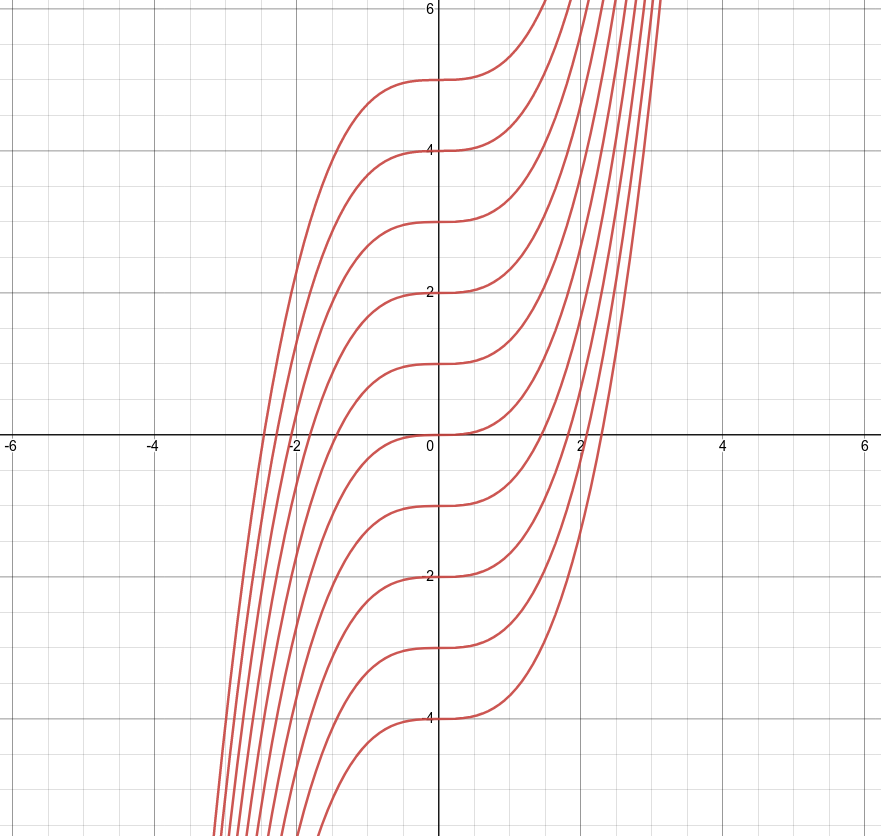
\includegraphics[scale=0.265]{section3-9_antiderivates1.png}
		\caption{Several Antiderivatives of $f(x)=x^2$, that is $\frac{x^3}{3} + C$}
		\end{subfigure}
		\hfill
		\begin{subfigure}[b]{0.49\textwidth}
		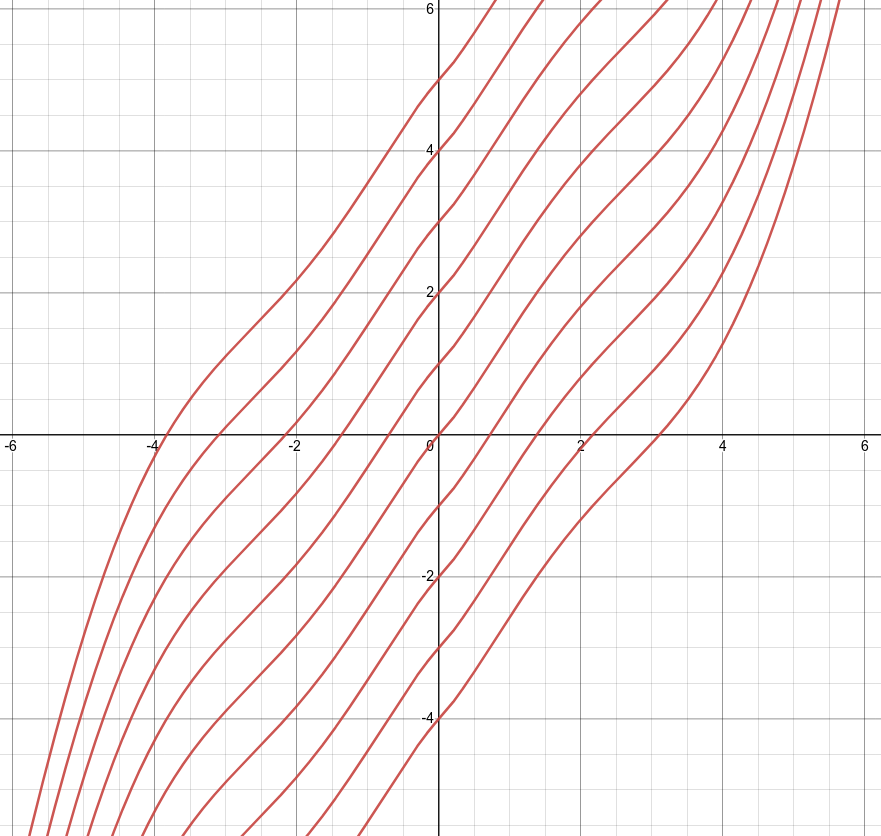
\includegraphics[scale=0.265]{section3-9_antiderivates.png}
		\caption{Several antiderivatives of $f(x) = x^{2/3} + \cos (x)$, that is $\frac{3}{5} x^{5/3} + \sin (x) + C$.}
		\end{subfigure}
	\end{figure}
	
	\vspace*{16pt}
	
	\begin{example}
	Find the most general antiderivative of each of the following functions.
	\begin{multicols}{3}
		\begin{enumerate}[label=\textbf{(\alph*)}]
		\item $f(x) = \sin x$.
		\item $f(x) = x^n$, $n \geq 0$.
		\end{enumerate}
	\end{multicols}
	\end{example}
	
	\newpage
	
	\section{Table of Antiderivatives}
	
	\begin{figure}[ht]
	\centering
	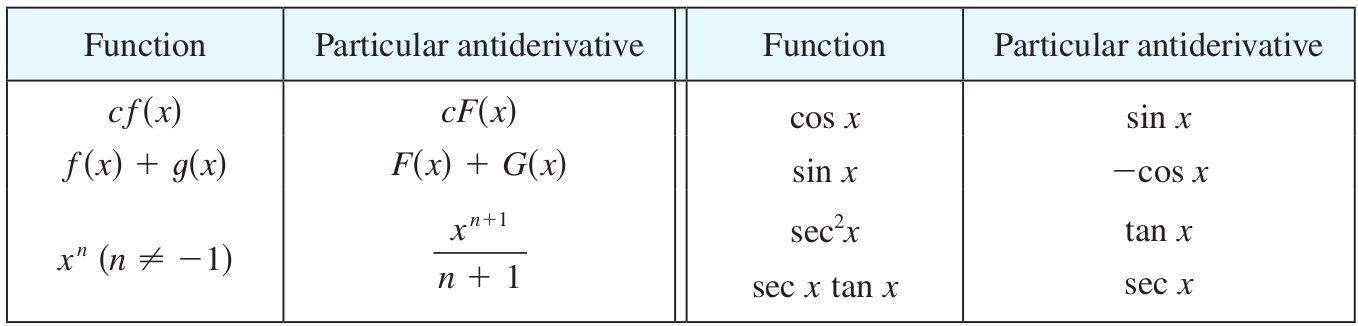
\includegraphics[scale=0.35]{section3-9_table.png}
	\caption{Properties and some Antiderivatives}
	\end{figure}
	
	\vspace*{20pt}
	
	\begin{example}
	Find all functions $g$ such that
		\begin{align*}
		g'(x) = 4 \sin x + \frac{2x^5 - \sqrt{x}}{x}.
		\end{align*}
	\end{example}
	
	\newpage
	
	\section{Initial Condition}	
	
	\begin{example}
	Find $F$ if $F'(x) = x \sqrt{x}$ and $F(1) = 2$.
	\end{example}
	
	\vfill
	
	\begin{example}
	Find $F$ if $F'(x) = \frac{1}{x^2}$ and $F(1) = 2$.
	\end{example}
	
	\vfill
	
	\newpage
	
	
	
	

\end{document}